\documentclass[11pt]{standalone}
\usepackage{tikz}
\usetikzlibrary{shapes.geometric}
\usetikzlibrary{plotmarks,shapes.multipart}
\usetikzlibrary{arrows.meta,calc,decorations.pathmorphing}
\begin{document} 

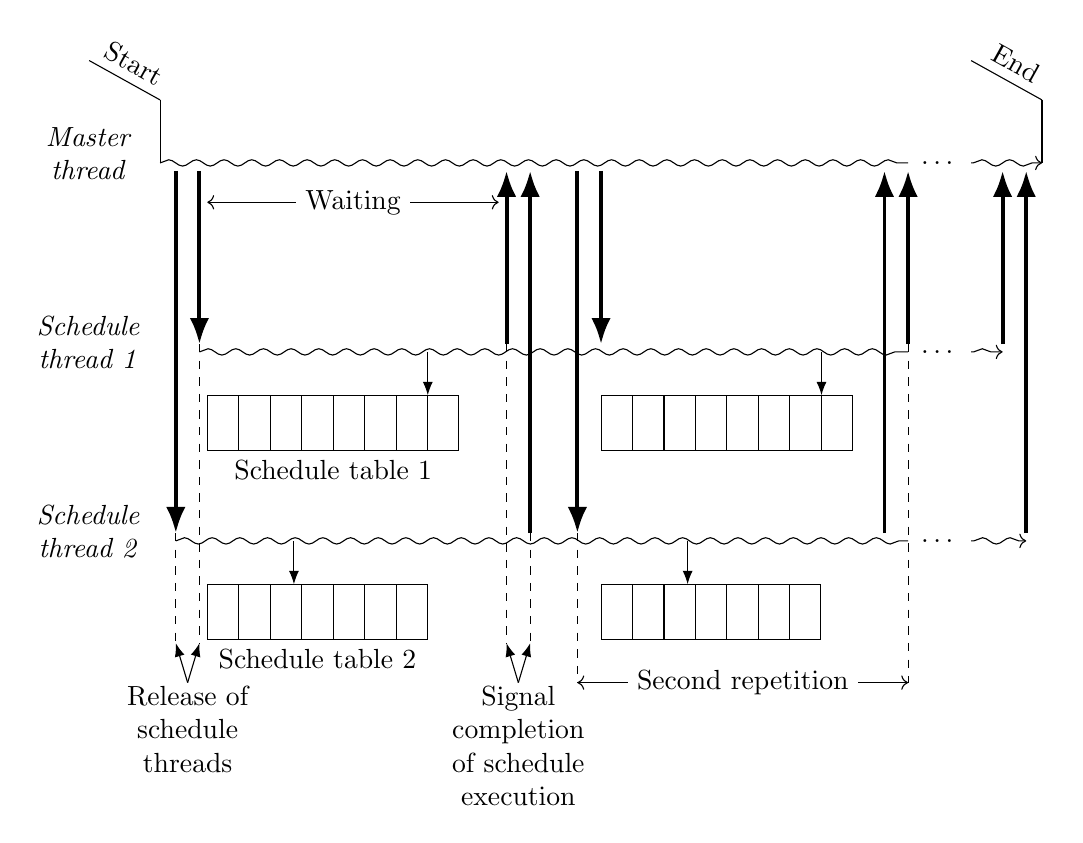
\begin{tikzpicture}


\node at(-2.5cm,-3.9cm) [label={[align=center,yshift=.7cm]south:\textit{Master}\\\textit{thread}}]{};
\draw [decorate,decoration={snake,pre=curveto,pre length=1,post length=1,amplitude=.4mm}] (-1.6cm,-3.9cm) -- (7.9cm,-3.9cm);


\node at(-2.5cm,-6.3cm) [label={[align=center,yshift=.7cm]south:\textit{Schedule}\\\textit{thread 1}}]{};
%\node at(0cm,-6cm) [rectangle, minimum width=6cm,minimum height=1.4cm,label={[anchor=west, yshift=-.3cm]west:{\textit{thread 1}}}] {};
\node at(-1cm,0) [rectangle split,rectangle split horizontal,rectangle split parts=8,anchor=west, draw, minimum width=5.6cm,minimum height=.7cm,yshift=-7.2cm, label={[align=center]south:Schedule table 1}]{};
\draw [decorate,decoration={snake,pre=curveto,pre length=1,post length=1,amplitude=.4mm}] (-1.1cm,-6.3cm) -- (7.9cm,-6.3cm);
\draw [-{Latex[]}] (1.8cm,-6.3cm) -- (1.8cm,-6.85cm);

\node at(-2.5cm,-8.7cm) [label={[align=center,yshift=.7cm]south:\textit{Schedule}\\\textit{thread 2}}]{};
%\node at(0cm,-8.4cm) [rectangle, minimum width=6cm,minimum height=1.4cm,label={[anchor=west, yshift=-.3cm]west:{\textit{thread 2}}}]{};
\node at(-1cm,0) [rectangle split,rectangle split horizontal,rectangle split parts=7,anchor=west, draw, minimum width=5.6cm,minimum height=.7cm,yshift=-9.6cm, label={[align=center]south:Schedule table 2}]{};
\draw [decorate,decoration={snake,pre=curveto,pre length=1,post length=1,amplitude=.4mm}] (-1.4cm,-8.7cm) -- (7.9cm,-8.7cm);
\draw [-{Latex[]}] (.1cm,-8.7cm) -- (.1cm,-9.25cm);

\path (-1.1cm,-4cm) edge[-{Latex[]},line width=.05cm] (-1.1cm,-6.2cm);
\path (-1.4cm,-4cm) edge[-{Latex[]},line width=.05cm] (-1.4cm,-8.6cm);

\path (2.8cm,-6.2cm) edge[-{Latex[]},line width=.05cm] (2.8cm,-4cm);
\path (3.1cm,-8.6cm) edge[-{Latex[]},line width=.05cm] (3.1cm,-4cm);



\node at(4cm,0) [rectangle split,rectangle split horizontal,rectangle split parts=8,anchor=west, draw, minimum width=5.6cm,minimum height=.7cm,yshift=-7.2cm]{};
\draw [-{Latex[]}] (6.8cm,-6.3cm) -- (6.8cm,-6.85cm);


\node at(4cm,0) [rectangle split,rectangle split horizontal,rectangle split parts=7,anchor=west, draw, minimum width=5.6cm,minimum height=.7cm,yshift=-9.6cm]{};
\draw [-{Latex[]}] (5.1cm,-8.7cm) -- (5.1cm,-9.25cm);

\path (4cm,-4cm) edge[-{Latex[]},line width=.05cm] (4cm,-6.2cm);
\path (3.7cm,-4cm) edge[-{Latex[]},line width=.05cm] (3.7cm,-8.6cm);

\path (7.9cm,-6.2cm) edge[-{Latex[]},line width=.05cm] (7.9cm,-4cm);
\path (7.6cm,-8.6cm) edge[-{Latex[]},line width=.05cm] (7.6cm,-4cm);

%\node [fill=white] at (-1.5cm,-4.8cm) {Startup};

\node at (8.3cm,-3.9cm) {\ldots};
\draw [->,decorate,decoration={snake,pre=curveto,pre length=1,post length=1,amplitude=.4mm}] (8.7cm,-3.9cm) -- (9.6cm,-3.9cm);
\node at (8.3cm,-6.3cm) {\ldots};
\draw [->,decorate,decoration={snake,pre=curveto,pre length=1,post length=1,amplitude=.4mm}] (8.7cm,-6.3cm) -- (9.1cm,-6.3cm);
\node at (8.3cm,-8.7cm) {\ldots};
\draw [->,decorate,decoration={snake,pre=curveto,pre length=1,post length=1,amplitude=.4mm}] (8.7cm,-8.7cm) -- (9.4cm,-8.7cm);

\path (9.1cm,-6.2cm) edge[-{Latex[]},line width=.05cm] (9.1cm,-4cm);
\path (9.4cm,-8.6cm) edge[-{Latex[]},line width=.05cm] (9.4cm,-4cm);

\draw [<->] (-1cm,-4.4cm) -- node[fill=white] {Waiting} (2.7cm,-4.4cm);
%-----------------------------------------------------
\draw [dashed] (-1.4cm,-8.6cm) -- (-1.4cm,-10cm); 
\draw [dashed] (-1.1cm,-6.2cm) -- (-1.1cm,-10cm); 

\draw [-{Latex[]}] (-1.25cm,-10.5cm) -- (-1.4cm,-10cm);
\draw [-{Latex[]}] (-1.25cm,-10.5cm) -- (-1.1cm,-10cm);

\node at(-1.25cm,-10.7cm) [label={[align=center,yshift=.4cm,text width=2cm]south:Release of schedule threads}]{};
%-----------------------------------------------------
\draw [dashed] (3.1cm,-8.6cm) -- (3.1cm,-10cm); 
\draw [dashed] (2.8cm,-6.2cm) -- (2.8cm,-10cm); 

\draw [-{Latex[]}] (2.95cm,-10.5cm) -- (3.1cm,-10cm);
\draw [-{Latex[]}] (2.95cm,-10.5cm) -- (2.8cm,-10cm);

\node at(2.95cm,-10.7cm) [label={[align=center,yshift=.4cm,text width=2cm]south:Signal completion of schedule execution}]{};

%----------------------------------------------------

\draw [dashed] (3.7cm,-8.6cm) -- (3.7cm,-10.5cm); 
\draw [dashed] (7.9cm,-6.2cm) -- (7.9cm,-10.5cm);

\draw [<->] (3.7cm,-10.5cm) -- node[fill=white] {Second repetition} (7.9cm,-10.5cm);

%------------------------------------------------------

\draw (-1.6cm,-3.9cm) -- (-1.6cm,-3.1cm);
\draw (-1.6cm,-3.1cm) -- node [sloped, anchor=center, above,] {Start} (-2.5cm,-2.6cm);

\draw (9.6cm,-3.9cm) -- (9.6cm,-3.1cm);
\draw (9.6cm,-3.1cm) -- node [sloped, anchor=center, above,] {End} (8.7cm,-2.6cm);

\end{tikzpicture}
\end{document}